\documentclass{article}
\usepackage{neurips_2026}

\usepackage[utf8]{inputenc}
\usepackage[T1]{fontenc}
\usepackage[bookmarks=false,breaklinks=true,pageanchor=false,pdfborder={0 0 0}]{hyperref}
\usepackage{url}
\usepackage{booktabs}
\usepackage{amsfonts}
\usepackage{amsmath}
\usepackage{amsthm}
\usepackage{nicefrac}
\usepackage{microtype}
\usepackage{xcolor}
\usepackage{graphicx}
\usepackage{caption}
\usepackage{subcaption}
\usepackage{multirow}
\usepackage{array}
\usepackage{tikz}
\usetikzlibrary{positioning,arrows.meta,shapes.geometric,fit,backgrounds,calc}

\definecolor{palTeal}{HTML}{1b9e77}
\definecolor{palOrange}{HTML}{d95f02}
\definecolor{palPurple}{HTML}{7570b3}
\definecolor{palPink}{HTML}{e7298a}
\definecolor{palGreen}{HTML}{66a61e}
\definecolor{palGold}{HTML}{e6ab02}
\definecolor{stageBg}{HTML}{f4f5f7}

\newtheorem{proposition}{Proposition}
\newtheorem{assumption}{Assumption}

\title{Does Confidence Track Visibility? Diagnosing Blind \\
Confidence in Cloud-Occluded Flood Segmentation}

\author{
  Anonymous Author(s) \\
  Affiliation \\
  Address \\
  \texttt{email}
}

\begin{document}

\maketitle

\begin{abstract}
Optical flood-mapping models are least reliable exactly when they are most needed: heavy cloud cover coincides with the monsoon and cyclone seasons that produce the floods these models must detect. We ask a narrow, falsifiable question -- does a model's predicted confidence track the real information loss from cloud occlusion, or does it stay artificially high as actual skill collapses? We build a controlled cloud-severity ladder over real Sentinel-1/Sentinel-2 chips from Sen1Floods11 and evaluate four flood classifiers -- an optical U-Net, a cloud-invariant SAR U-Net, an early-fusion SAR+optical U-Net, and a classical NDWI rule -- across seven severities. The optical model's confidence-minus-accuracy gap (GapAUC) is significantly positive ($+0.047$, 95\% CI $[+0.027,+0.070]$, $n=64$ test chips), while SAR's gap is an order of magnitude smaller, exactly as its cloud-invariant design predicts. Water-class IoU shows this understates the damage: raw accuracy suggests mild optical degradation, while IoU collapses from $0.457$ to $0.146$. A false-negative/false-positive decomposition shows the fusion model's apparently good calibration masks a different failure -- a sharp rise in false alarms, not missed detections, under heavy cloud. Finally, a per-severity selective-prediction layer targeting a 10\% missed-flood rate certifies no threshold at any severity for any model, a negative result we attribute to insufficient model accuracy at pilot scale, not the calibration procedure. Code and configuration: \url{https://anonymous.4open.science/r/blind-confidence-flood-XXXX}.
\end{abstract}

\section{Introduction}
\label{sec:intro}

Flooding affects more people than any other environmental hazard, and satellite-observed flood extent grew by roughly a quarter of exposed global population between 2000 and 2015 \citep{tellman2021satellite}. Optical sensors like Sentinel-2 give flood models rich spectral information, but it disappears under cloud -- and cloud cover is not an occasional nuisance here, it is systematically worst during the meteorological conditions (monsoons, tropical cyclones) that cause the floods being mapped. SAR sensors like Sentinel-1 penetrate cloud and are the operational standard for this reason \citep{misra2025mapping}, but optical imagery remains widely used where spectral resolution or existing pipelines favor it, and hybrid fusion of both modalities is an active research area.

This creates a specific, checkable failure mode distinct from ``the model gets less accurate under cloud'' -- a fact no one disputes. The question is whether the model's own confidence \emph{knows} this is happening. A system that silently degrades but keeps reporting high confidence is more dangerous than one that says so, since the former gives operators no signal to fall back to a cloud-invariant source or a human reviewer. This is the failure mode documented for deep networks generally \citep{guo2017calibration} and under distribution shift specifically \citep{ovadia2019trust}, and a natural instance of the corruption-robustness setting studied by \citet{hendrycks2019benchmarking} -- except the corruption here is real and physically motivated, not synthetic noise on a benchmark image.

We make four contributions. \textbf{(1)} We adapt a confidence-versus-visibility diagnostic, originally built for degradation ladders in vision-language models, to a real Earth-observation task with a physically motivated severity axis, validated against a genuine cloud-invariant control (SAR) rather than only a corrupted-input baseline. \textbf{(2)} We show raw pixel accuracy substantially understates the real collapse in flood-detection skill under cloud, and that water-class IoU is necessary to see it. \textbf{(3)} We decompose failure into false negatives and false positives and show SAR-optical fusion's apparently good calibration compounds two effects moving in different directions, not genuine robustness -- more actionable than a simple accuracy comparison. \textbf{(4)} We attempt a distribution-free selective-prediction layer with a finite-sample missed-flood guarantee, report its complete failure to certify any threshold, and diagnose why rather than treating the negative result as a bug to hide.

We report this work at pilot scale throughout: three lightweight U-Nets, 316 usable chips, a single T4 GPU -- a strength for the workshop's interest in ground-up, resource-constrained methodology, not a limitation to apologize for, but we are correspondingly careful not to claim more generality than 316 chips across ten flood events can support.

\section{Related Work}
\label{sec:related}

\textbf{Flood mapping and multi-sensor benchmarks.} Sen1Floods11 \citep{bonafilia2020sen1floods11} is the primary hand-labeled benchmark pairing Sentinel-1/-2 with flood-water ground truth, and is the dataset we build on. \citet{misra2025mapping} deploy a SAR-only global flood model precisely because SAR is unaffected by cloud, and \citet{tellman2021satellite} establish the scale of the exposure problem motivating reliable mapping.

\textbf{Calibration and selective prediction.} \citet{guo2017calibration} and \citet{minderer2021revisiting} document systematic overconfidence; \citet{ovadia2019trust} show this worsens under distribution shift -- exactly the regime a severity ladder induces. Selective classification \citep{geifman2017selective} and distribution-free risk control \citep{bates2021distribution} give the machinery for turning confidence into an abstention rule with a finite-sample guarantee, adopted directly here.

\textbf{Corruption robustness.} Our ladder is methodologically closest to \citet{hendrycks2019benchmarking}, who benchmark robustness against a fixed taxonomy of synthetic corruptions; ours is designed to be physically motivated rather than an arbitrary filter, and validated against a real cloud-invariant sensor rather than accuracy degradation alone.

\section{Method}
\label{sec:method}

\textbf{Severity ladder.} For a chip's optical bands $x \in [0,1]^{13 \times H \times W}$, we generate a smooth opacity field $c_s \in [0,1]^{H\times W}$ via multi-octave value noise, thresholded so $\mathbb{E}[c_s] \approx s$ for target severity $s \in \mathcal{S} = \{0, 0.15, \ldots, 0.90\}$, and composite $\tilde x = x \odot (1-c_s) + \kappa\, c_s$ toward a bright cloud-reflectance constant $\kappa$. Radar bands are never touched by $c_s$, which makes the SAR model a genuine control, not another treatment arm.

\textbf{Models.} We train three lightweight U-Nets \citep{ronneberger2015unet} with a ResNet-18 encoder \citep{he2016deep}, ImageNet-initialized when reachable \citep{deng2009imagenet}, differing only in input channels: \textsc{sar} (VV, VH), \textsc{optical} (blue, green, red, NIR), and \textsc{fusion} (both, early-concatenated). All three are trained identically -- masked binary cross-entropy plus Dice loss \citep{milletari2016vnet} on \emph{clean} (severity-0) chips only, AdamW \citep{loshchilov2019decoupled}, 20 epochs -- so that any behavioral difference under synthetic cloud at test time is attributable to architecture and input modality, not to differential exposure to corrupted training data. A fourth, non-learned baseline applies the classical NDWI rule \citep{mcfeeters1996ndwi} directly to the (possibly cloud-composited) optical bands.

\textbf{The GapAUC diagnostic.} For model $f$, let $\bar c_f(s)$ and $\mathrm{Acc}_f(s)$ denote mean predicted confidence and pixel accuracy at severity $s$ over held-out chips. We define
\begin{equation}
\label{eq:gapauc}
\mathrm{GapAUC}(f) \;=\; \int_0^{s_{\max}} \big[\bar c_f(s) - \mathrm{Acc}_f(s)\big]\, ds \;\approx\; \sum_{i} \tfrac{1}{2}\big(g_f(s_i) + g_f(s_{i+1})\big)(s_{i+1}-s_i),
\end{equation}
with $g_f(s) = \bar c_f(s) - \mathrm{Acc}_f(s)$, estimated by the trapezoidal rule over $\mathcal S$. $\mathrm{GapAUC}(f) \approx 0$ means confidence tracks real, severity-dependent competence; $\mathrm{GapAUC}(f) \gg 0$ is the blind-confidence signature. CIs resample whole chips (not pixels) $2{,}000$ times, respecting the true unit of independence; pairwise comparisons use a $20{,}000$-permutation test on chip-clustered gap series with Bonferroni correction across the three comparisons against optical.

\textbf{Selective prediction.} We additionally ask whether confidence can be turned into an operationally useful abstention rule with a finite-sample guarantee. Fix severity $s$ and threshold $\tau$; call a calibration chip \emph{trusted} if $\bar c_i(s)\ge\tau$ and \emph{missed} if a majority of its true flood pixels are false negatives. Proposition~\ref{prop:selective} (Appendix~\ref{app:stats}) shows that if the Clopper--Pearson upper $(1-\alpha)$ bound \citep{clopper1934use} on the empirical missed-chip rate among trusted calibration chips is at most $\delta$, then, under calibration/test exchangeability, the true missed-chip rate among trusted \emph{test} chips is at most $\delta$ with probability $\ge 1-\alpha$. We search for the lowest threshold certifying $\delta\le0.10$ at $\alpha=0.05$, \emph{separately per severity} -- a strictly weaker, more achievable requirement than certifying one threshold across all seven severities simultaneously, which an earlier version of this pipeline attempted and which is mathematically close to unreachable at pilot scale (Appendix~\ref{app:h3}).

\section{Experiments}
\label{sec:experiments}

\textbf{Data.} We pool Sen1Floods11's official train/validation/test splits into one candidate set of 431 hand-labeled chips spanning ten flood events on five continents, then apply our own random $60/20/20$ re-split (fixed seed) after discarding 4 chips with no valid ground-truth pixels, leaving 316: 189 train, 63 validation, 64 test. Each chip is $512\times512$ px resized to $256\times256$; Sentinel-2 bands are TOA-reflectance-normalized to $[0,1]$, Sentinel-1 clipped to $[-30,0]$ dB and rescaled (Appendix~\ref{app:data}).

\textbf{Setup.} All three U-Nets and NDWI are evaluated identically across $\mathcal S$ on the 64 test chips; training all three took $103$ seconds total on one T4 GPU.

\begin{table}[t]
\centering
\caption{GapAUC (Eq.~\ref{eq:gapauc}) by model: 2{,}000-resample bootstrap 95\% CIs, Bonferroni-adjusted permutation $p$ vs.\ optical ($n{=}64$, $\alpha_{\text{adj}}=0.0167$). SAR's near-zero gap validates the ladder itself, not just the optical model's failure.}
\label{tab:gapauc}
\small
\renewcommand{\arraystretch}{0.92}
\begin{tabular}{lccc}
\toprule
Model & GapAUC & 95\% CI & $p$ vs.\ optical \\
\midrule
Optical U-Net           & $+0.047$ & $[+0.027,\,+0.070]$ & -- \\
SAR U-Net                & $+0.014$ & $[+0.006,\,+0.025]$ & $0.0056$ \\
SAR+Optical U-Net (fusion) & $+0.006$ & $[-0.001,\,+0.013]$ & $<0.001$ \\
NDWI (rule-based)        & $-0.566$ & $[-0.583,\,-0.551]$ & $<0.001$ \\
\bottomrule
\end{tabular}
\end{table}

\textbf{H1: the optical model is blind-confident.} Table~\ref{tab:gapauc} shows GapAUC significantly above zero for the optical model, CI excluding zero by a wide margin. Figure~\ref{fig:panel1} visualizes the mechanism: as severity rises from 0 to 0.9, optical accuracy declines only modestly (Table~\ref{tab:accuracy}: $0.955 \to 0.914$) while confidence barely moves -- but water-class IoU, isolating real flood-detection skill from the majority non-water class, collapses from $0.457$ to $0.146$ (Table~\ref{tab:iou}). Raw accuracy is class-imbalance-prone and materially understates the real damage; IoU reveals it.

\begin{figure}[t]
  \centering
  
\includegraphics[width=0.95\linewidth]{figures/fig1_panel_overview.pdf}
  \caption{(a--d) Accuracy, confidence, gap, and GapAUC-with-significance across the cloud-severity ladder, all four models, 64-chip test set. Shading in (c) visualizes the gap; asterisks in (d) mark Bonferroni-significant differences from optical. SAR (orange) is essentially flat throughout, exactly as its cloud-invariant design predicts.}
  \label{fig:panel1}
\end{figure}

\textbf{H2: SAR is a clean control; fusion's good calibration is not what it looks like.} SAR's GapAUC is an order of magnitude smaller than optical's and its accuracy is exactly flat across all seven severities ($0.959$ throughout) -- the sanity check a synthetic-corruption study needs, since SAR bands are never touched by the cloud compositor. Fusion's GapAUC ($+0.006$, CI includes zero) looks best-calibrated of the three. Table~\ref{tab:accuracy}, however, shows fusion's own accuracy and water-IoU collapsing \emph{more} severely than optical's under heavy cloud ($0.968\to0.602$ accuracy, $0.498\to0.093$ IoU) -- fusion is well-calibrated \emph{and} the least useful model at $s=0.9$, which a confidence-tracking metric alone cannot distinguish from genuine robustness. A false-negative/false-positive decomposition (Appendix~\ref{app:fnfp}, Fig.~\ref{fig:fnfp}) clarifies the mechanism: fusion's false-negative rate at high severity is comparable to or lower than optical's, but its false-positive rate rises sharply -- exposed to a corrupted optical branch it was never trained to discount, the model increasingly hallucinates flood water rather than missing it. One caveat: fusion's best validation checkpoint was epoch 18/20, still improving, so this should be confirmed with longer training before being read as architectural rather than a training artifact (Appendix~\ref{app:training}).

\begin{table}[t]
\centering
\caption{Pixel accuracy and water-class IoU/F1 at three representative severities ($n{=}64$).}
\label{tab:accuracy}
\label{tab:iou}
\footnotesize
\renewcommand{\arraystretch}{0.92}
\begin{tabular}{lccc@{\hspace{1.2em}}ccc}
\toprule
& \multicolumn{3}{c}{Pixel accuracy} & \multicolumn{3}{c}{Water-class IoU / F1} \\
\cmidrule(lr){2-4} \cmidrule(lr){5-7}
Model & $s{=}0$ & $s{=}0.45$ & $s{=}0.9$ & $s{=}0$ & $s{=}0.45$ & $s{=}0.9$ \\
\midrule
Optical & 0.955 & 0.931 & 0.914 & 0.457/0.548 & 0.216/0.265 & 0.146/0.151 \\
SAR & 0.959 & 0.959 & 0.959 & 0.369/0.453 & 0.369/0.453 & 0.369/0.453 \\
Fusion & 0.968 & 0.906 & 0.602 & 0.498/0.597 & 0.136/0.198 & 0.093/0.140 \\
NDWI & 0.966 & 0.966 & 0.966 & 0.460/0.538 & 0.460/0.538 & 0.460/0.538 \\
\bottomrule
\end{tabular}
\end{table}

\textbf{H3: selective prediction fails to certify -- and we know why.} Across all seven severities and all four models, zero threshold-severity combinations certify the target $10\%$ missed-flood rate ($n_{\text{certified}}=0/7$ for every model; Appendix~\ref{app:h3}). This design is strictly more achievable than an earlier, cross-severity version requiring one threshold across all conditions at once; persistence with $63$ calibration chips -- above the $\sim\!30$-chip floor a Clopper-Pearson bound needs in the best case (Appendix~\ref{app:powercalc}) -- indicates the binding constraint is model accuracy, not calibration-sample size. We report this as an informative negative result: no model's most-confident region is accurate enough to certify a $10\%$ guarantee at this scale, and calibration engineering will not change that.

\textbf{Generalization across events.} Appendix~\ref{app:events} (Fig.~\ref{fig:events}) breaks GapAUC down by the ten flood events in the test set. Nine of the ten yield a clearly positive point estimate for the optical model, ranging from small to substantially larger in Nigeria and the Mekong basin; the tenth, Somalia, has only $n{=}2$ chips and sits at essentially zero rather than clearly on either side. Per-event counts are small ($n{=}2$ to $12$), so we read this as directional consistency rather than a per-event significance claim.

\section{Limitations, Broader Impact, and Conclusion}
\label{sec:limitations}
This is a pilot study throughout. Two points, with full discussion in the appendix given space: our synthetic cloud composite has a verified mathematical property that makes NDWI's flat accuracy a compositing-scheme artifact, not genuine robustness (Appendix~\ref{app:cloudmech}), and the strong GapAUC--water-fraction link we find (Appendix~\ref{app:waterfrac}, Spearman $\rho=0.98$, $p<0.001$) is partly confounded by accuracy's metric properties, not a clean causal effect. All findings are specific to lightweight U-Nets trained 20 epochs on 189 chips.

In sum: optical confidence does not track real competence loss under cloud -- visible via IoU but not accuracy; fusion's good calibration can mask a shift toward false alarms rather than genuine robustness; and a certified abstention rule is harder to build than a diagnostic. Code released for reproducibility (Appendix~\ref{app:repro}).

\bibliographystyle{plainnat}
\bibliography{references}

\clearpage
\appendix
\section*{Appendix}
This appendix is organized so that each section is self-contained and can be read independently of the others. Section~\ref{app:overview} gives a one-page visual overview of the full pipeline; Section~\ref{app:data} gives full dataset and preprocessing detail; Section~\ref{app:cloudmech} documents a verified mechanistic property of the synthetic cloud model; Section~\ref{app:training} gives architecture, optimization, and compute detail; Section~\ref{app:stats} gives the full statistical methodology, including the formal statement and proof of Proposition~\ref{prop:selective}; Sections~\ref{app:h3}--\ref{app:extra_figures} give the complete results behind every claim summarized in the main text; Section~\ref{app:hyperparams} is a single consolidated hyperparameter and reproducibility table; Section~\ref{app:repro} is a reproducibility statement; Section~\ref{app:impact} closes with broader impact.

\section{Pipeline Overview}
\label{app:overview}

Figure~\ref{fig:pipeline} lays out the full pipeline end to end, from raw chips to the three headline findings, as a single reference diagram. Every stage is described in full in the sections that follow; this figure exists so a reader can hold the whole design in mind before working through the details.

\begin{figure}[h]
\centering
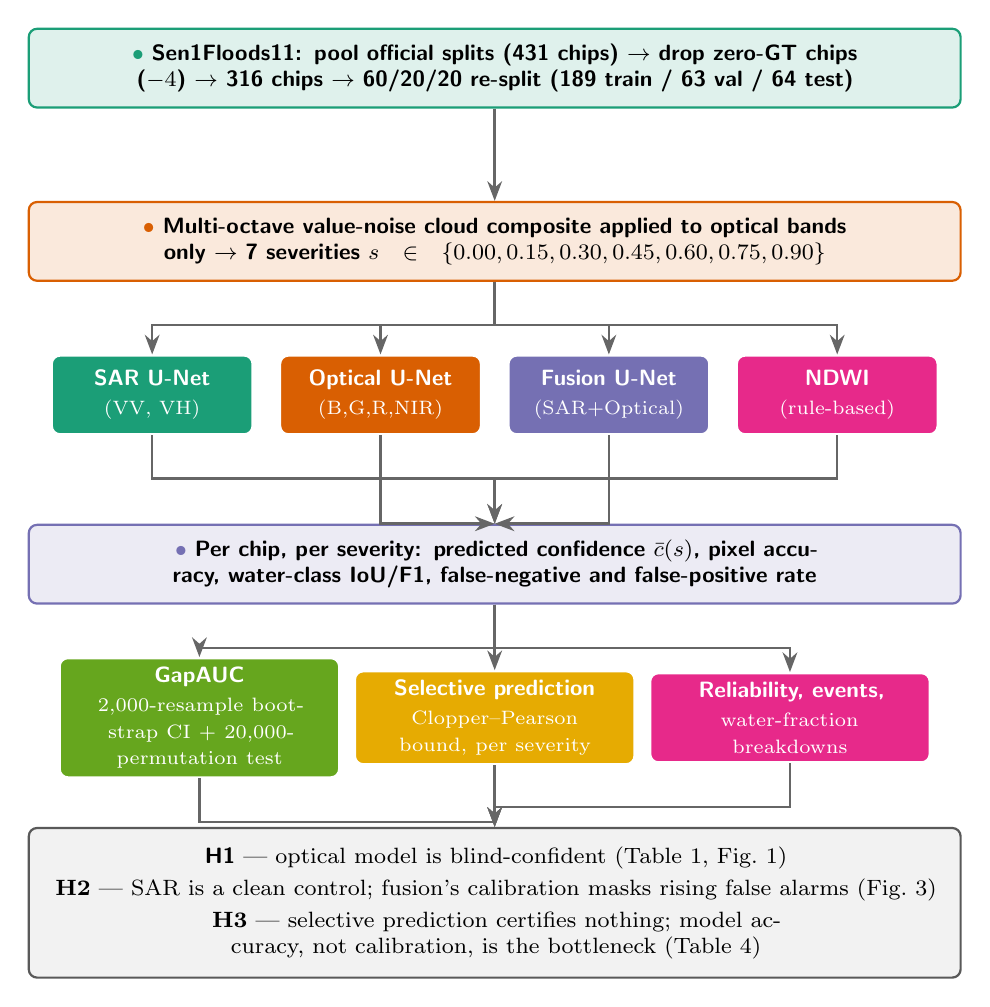
\begin{tikzpicture}[
  font=\sffamily,
  every node/.style={align=center},
  wide/.style={rectangle, rounded corners=3pt, draw=black!55, thick,
    minimum height=1.0cm, text width=11.6cm, align=center, fill=stageBg,
    font=\sffamily\bfseries\footnotesize},
  model/.style={rectangle, rounded corners=3pt, draw=white, thick,
    minimum height=1.0cm, minimum width=2.55cm, align=center,
    font=\sffamily\bfseries\footnotesize, text=white},
  arr/.style={-{Stealth[length=2.5mm]}, line width=0.9pt, draw=black!60}
]

\node[wide, fill=palTeal!14, draw=palTeal] (data) at (0,0)
  {\textcolor{palTeal}{$\bullet$}~Sen1Floods11: pool official splits (431 chips) $\rightarrow$ drop zero-GT chips ($-4$) $\rightarrow$ 316 chips $\rightarrow$ 60/20/20 re-split (189 train / 63 val / 64 test)};

\node[wide, fill=palOrange!14, draw=palOrange] (deg) at (0,-2.2)
  {\textcolor{palOrange}{$\bullet$}~Multi-octave value-noise cloud composite applied to optical bands only $\rightarrow$ 7 severities $s \in \{0.00, 0.15, 0.30, 0.45, 0.60, 0.75, 0.90\}$};
\draw[arr] (data.south) -- (deg.north);

\node[model, fill=palTeal]   (sar)  at (-4.35,-4.15) {SAR U-Net\\[1pt]\scriptsize\normalfont (VV, VH)};
\node[model, fill=palOrange] (opt)  at (-1.45,-4.15) {Optical U-Net\\[1pt]\scriptsize\normalfont (B,G,R,NIR)};
\node[model, fill=palPurple] (fus)  at ( 1.45,-4.15) {Fusion U-Net\\[1pt]\scriptsize\normalfont (SAR+Optical)};
\node[model, fill=palPink]   (ndwi) at ( 4.35,-4.15) {NDWI\\[1pt]\scriptsize\normalfont (rule-based)};

\draw[arr] (deg.south) -- ++(0,-0.55) -| (sar.north);
\draw[arr] (deg.south) -- ++(0,-0.55) -| (opt.north);
\draw[arr] (deg.south) -- ++(0,-0.55) -| (fus.north);
\draw[arr] (deg.south) -- ++(0,-0.55) -| (ndwi.north);

\node[wide, fill=palPurple!14, draw=palPurple] (metrics) at (0,-6.3)
  {\textcolor{palPurple}{$\bullet$}~Per chip, per severity: predicted confidence $\bar c(s)$, pixel accuracy, water-class IoU/F1, false-negative and false-positive rate};

\draw[arr] (sar.south)  -- ++(0,-0.55) -| (metrics.north);
\draw[arr] (opt.south)  -- ++(0,-0.4)  |- (metrics.north);
\draw[arr] (fus.south)  -- ++(0,-0.4)  |- (metrics.north);
\draw[arr] (ndwi.south) -- ++(0,-0.55) -| (metrics.north);

\node[model, text width=3.1cm, minimum width=3.55cm, fill=palGreen] (gapauc) at (-3.75,-8.25)
  {GapAUC\\[1pt]\scriptsize\normalfont 2{,}000-resample bootstrap CI + 20{,}000-permutation test};
\node[model, text width=3.1cm, minimum width=3.55cm, fill=palGold] (selpred) at (0,-8.25)
  {Selective prediction\\[1pt]\scriptsize\normalfont Clopper--Pearson bound, per severity};
\node[model, text width=3.1cm, minimum width=3.55cm, fill=palPink] (extra) at (3.75,-8.25)
  {Reliability, events,\\[1pt]\scriptsize\normalfont water-fraction breakdowns};

\draw[arr] (metrics.south) -- ++(0,-0.55) -| (gapauc.north);
\draw[arr] (metrics.south) -- ++(0,-0.55) -| (selpred.north);
\draw[arr] (metrics.south) -- ++(0,-0.55) -| (extra.north);

\node[wide, minimum height=1.9cm, fill=black!5, draw=black!65] (findings) at (0,-10.6)
  {\bfseries H1 \normalfont --- optical model is blind-confident (Table 1, Fig.\ 1) \\[2pt]
   \bfseries H2 \normalfont --- SAR is a clean control; fusion's calibration masks rising false alarms (Fig.\ 3) \\[2pt]
   \bfseries H3 \normalfont --- selective prediction certifies nothing; model accuracy, not calibration, is the bottleneck (Table 4)};

\draw[arr] (gapauc.south)  -- ++(0,-0.55) -| (findings.north);
\draw[arr] (selpred.south) -- (findings.north);
\draw[arr] (extra.south)   -- ++(0,-0.55) -| (findings.north);

\end{tikzpicture}
\caption{End-to-end pipeline. Top to bottom: data pooling and filtering (Appendix~\ref{app:data}); the synthetic cloud-severity ladder (Appendix~\ref{app:cloudmech}); the four models evaluated identically at every severity (Appendix~\ref{app:training}); the per-chip metrics computed from each model's output; the three families of diagnostic analysis built on those metrics (Appendices~\ref{app:stats}--\ref{app:waterfrac}); and the three findings that follow. Colors are decorative groupings only and carry no quantitative meaning.}
\label{fig:pipeline}
\end{figure}

\section{Dataset and Preprocessing}
\label{app:data}

\subsection{Source and licensing}
We use Sen1Floods11 \citep{bonafilia2020sen1floods11}, a CC-BY-licensed, publicly available benchmark distributed by Cloud to Street and NASA. We use only the \texttt{HandLabeled} subset, in which every chip's flood/no-flood label was produced by manual annotation rather than automated thresholding.

\subsection{Band structure}
Table~\ref{tab:bands} summarizes the three raster layers used per chip, each a $512\times512$ pixel GeoTIFF at $10$m nominal resolution.

\begin{table}[h]
\centering
\caption{Sen1Floods11 HandLabeled raster layers.}
\label{tab:bands}
\begin{tabular}{lccl}
\toprule
Layer & Bands & Dtype & Notes \\
\midrule
\texttt{S1Hand} & 2 (VV, VH) & Float32 & dB units; no cloud sensitivity \\
\texttt{S2Hand} & 13 (B1--B12, B8A) & UInt16 & TOA reflectance $\times\,10{,}000$; \emph{no shipped cloud mask} \\
\texttt{LabelHand} & 1 & Int16 & $-1$ nodata, $0$ not-water, $1$ water \\
\bottomrule
\end{tabular}
\end{table}

We use Sentinel-2 band indices $\{1,2,3,7\}$ (Blue, Green, Red, NIR) as the four-channel optical input; NDWI uses Green and NIR directly. The absence of a shipped cloud mask is precisely why our severity ladder is a controlled synthetic composite rather than a filter on real cloud pixels; see the discussion of this design choice's limitations in the main text (Section~\ref{sec:limitations}) and the mechanism detail in Appendix~\ref{app:cloudmech}.

\subsection{Splits and chip filtering}
The official Sen1Floods11 handlabeled release ships \texttt{train}/\texttt{valid}/\texttt{test} split CSVs. Because the \texttt{valid} split alone contains only 89 chips -- too few to give the selective-prediction layer (Appendix~\ref{app:h3}) a realistic chance of certifying anything, independent of any modeling choice -- we pool all three official splits into one candidate set (431 unique chips after de-duplication) and perform our own random $60/20/20$ re-split with a fixed seed. This does not leak the official train/test boundary into our evaluation, since we never use the official split labels for anything other than chip discovery.

Four chips were excluded because their \texttt{LabelHand} layer contains no valid (non-nodata) pixels at all: \texttt{Ghana\_277}, \texttt{Ghana\_26376}, \texttt{Ghana\_234935}, \texttt{Ghana\_5079}. This filtering is applied once, upfront, from label data alone -- before any model is trained -- so that no model's behavior can influence which chips are considered valid. The resulting 316-chip pool splits into 189 train / 63 validation / 64 test chips, spanning ten flood events: Ghana, India, Mekong (Cambodia/Vietnam/Laos basin), Nigeria, Pakistan, Paraguay, Somalia, Spain, Sri Lanka, and USA.

\subsection{Preprocessing}
Sentinel-1 bands are clipped to $[-30, 0]$ dB and rescaled to $[0,1]$; any non-finite value (NaN or $-\infty$, which occurs in real Sentinel-1 GRD nodata regions) is mapped to the $-30$ dB floor \emph{before} clipping, since clipping alone does not sanitize non-finite values. Sentinel-2 bands are divided by $10{,}000$ and clipped to $[0,1]$. All chips are resized from $512\times512$ to $256\times256$ (bilinear for imagery, nearest-neighbor for labels, to preserve the exact $\{-1,0,1\}$ label alphabet) for T4 memory and time budget.

\section{Cloud-Occlusion Mechanism}
\label{app:cloudmech}

The opacity field $c_s$ (Section~\ref{sec:method}) is generated by summing five octaves of value noise at successive scales with geometrically decaying amplitude (ratio $0.55$) -- in the spirit of the procedural fractal-noise techniques introduced to computer graphics by \citet{perlin1985image}, though our construction uses interpolated random grids rather than gradient noise -- normalizing to $[0,1]$, and passing through a logistic function centered at the $(1-s)$-quantile of the field with slope $12$, which yields a smooth, spatially coherent mask whose mean opacity closely tracks the target severity $s$. Figure~\ref{fig:cloudladder} shows the resulting ladder on one chip, both as the raw opacity mask and composited onto true-color Sentinel-2 imagery with a $2$--$98$ percentile contrast stretch.

\begin{figure}[h]
  \centering
  
\includegraphics[width=\linewidth]{figures/figA4_cloud_ladder_illustration.pdf}
  \caption{The synthetic cloud-occlusion ladder, shown as the raw per-pixel opacity mask (top) and composited onto real Sentinel-2 RGB (bottom), for one representative chip across all seven severities used in the study.}
  \label{fig:cloudladder}
\end{figure}

\textbf{A mechanistic caveat we verified directly.} The compositing rule blends each band toward a single bright constant $\kappa$: $\tilde x = x(1-c_s) + \kappa c_s$. For any two bands $b_1, b_2$, their difference transforms as $\tilde b_1 - \tilde b_2 = (b_1 - b_2)(1-c_s)$ -- the sign of the difference is preserved for any $c_s < 1$, only its magnitude shrinks. Since NDWI's binary decision depends only on the \emph{sign} of Green$-$NIR, this means our specific linear compositing scheme cannot flip an NDWI decision through severity alone; it can only shrink the pseudo-confidence magnitude $|\mathrm{NDWI}|$. This exactly explains why NDWI's raw accuracy is flat across all severities (Table~\ref{tab:accuracy}) while its GapAUC is strongly negative (Table~\ref{tab:gapauc}: NDWI recognizes, correctly, that its confidence should collapse, even though our particular synthetic cloud does not actually degrade its classification decisions the way a physically heterogeneous real cloud would). We flag this as a concrete, verified limitation of the synthetic-cloud methodology rather than speculate about it.

\section{Model, Training, and Compute Detail}
\label{app:training}

\subsection{Architecture}
All three trained models are U-Nets \citep{ronneberger2015unet} with a ResNet-18 \citep{he2016deep} encoder, differing only in input channel count (SAR: 2, Optical: 4, Fusion: 6, all early-concatenated for the fusion case). Encoder weights are ImageNet-initialized \citep{deng2009imagenet} when reachable; our training code includes an automatic fallback to random initialization with a logged warning if pretrained weights cannot be downloaded, so that a network failure degrades gracefully rather than silently changing the experiment.

\subsection{Loss and optimization}
We minimize a per-pixel masked (nodata-excluded) sum of binary cross-entropy and Dice loss \citep{milletari2016vnet}, using AdamW \citep{loshchilov2019decoupled} -- Adam \citep{kingma2015adam} with weight decay decoupled from the gradient update -- at learning rate $10^{-3}$, weight decay $10^{-4}$, batch size $8$, for $20$ epochs, with mixed-precision training. All training uses only severity-$0$ (clean) chips; no model ever sees synthetic cloud during training, which is what makes test-time behavioral differences under cloud attributable to modality and architecture rather than differential training exposure.

\subsection{Training diagnostics}
We track each model's best validation-loss checkpoint epoch as a lightweight, automatic diagnostic against undertraining, and we additionally instrument training to halt immediately with an explicit error, rather than continue silently, if any epoch's loss becomes non-finite -- this was added after an earlier iteration of this pipeline let unsanitized non-finite Sentinel-1 values propagate into a model's weights undetected. In the run reported here: SAR's best checkpoint was epoch 15/20, optical's was epoch 13/20, and fusion's was epoch 18/20 -- still improving at the final epoch. We flag this explicitly wherever it is relevant to interpretation (Section~\ref{sec:experiments}, Appendix~\ref{app:fnfp}): fusion's false-positive-driven failure mode under heavy cloud should be confirmed with a longer training budget before being read as a stable architectural property rather than a training-time artifact.

\subsection{Compute}
Total training time for all three models was $103$ seconds wall-clock on a single NVIDIA T4 GPU (Google Colab/Kaggle-class free-tier hardware). Full evaluation across all seven severities, four models, and both validation and test splits adds a comparable amount of time. The complete pipeline -- data download, training, evaluation, all statistical tests, and all figures in this paper -- runs in well under one T4 GPU-hour. Table~\ref{tab:hyperparams} (Appendix~\ref{app:hyperparams}) consolidates every parameter mentioned across this appendix into a single reference.

\section{Statistical Methodology}
\label{app:stats}

\subsection{Bootstrap confidence intervals}
GapAUC confidence intervals (Table~\ref{tab:gapauc}) are constructed by resampling whole chips with replacement, $2{,}000$ times, and recomputing Equation~\ref{eq:gapauc} on each resample \citep{efron1993bootstrap}; we report the $2.5$/$97.5$ percentiles of the resulting distribution. Resampling chips rather than pixels respects the true unit of statistical independence -- pixels within a chip are highly spatially correlated, and treating them as independent would badly understate variance.

\subsection{Permutation tests and multiple comparisons}
Pairwise GapAUC comparisons against the optical model use a $20{,}000$-permutation test on the chip-level $(\text{confidence}-\text{accuracy})$ series, permuting chip labels between the two models being compared and recomputing the GapAUC difference each time. With three comparisons (optical vs.\ SAR, vs.\ fusion, vs.\ NDWI) we apply Bonferroni correction, testing at $\alpha_{\text{adj}} = 0.05/3 \approx 0.0167$. All three comparisons in Table~\ref{tab:gapauc} remain significant at this corrected level.

\subsection{Selective prediction: formal guarantee}
\label{app:proposition}

\begin{proposition}[Finite-sample missed-flood guarantee]
\label{prop:selective}
Let calibration chips at severity $s$ be exchangeable with test chips at severity $s$. Let $\hat p_\tau$ be the empirical missed-chip rate among $n_\tau$ trusted calibration chips (chips with $\bar c_i(s) \ge \tau$), and let $U_{1-\alpha}(\hat p_\tau, n_\tau)$ be the Clopper--Pearson upper $(1-\alpha)$ confidence bound \citep{clopper1934use} for a Binomial proportion. If $U_{1-\alpha}(\hat p_\tau, n_\tau) \le \delta$, then the true missed-chip rate among trusted \emph{test} chips at severity $s$ is at most $\delta$ with probability at least $1-\alpha$ over the calibration sample.
\end{proposition}

\begin{proof}
By definition, the Clopper--Pearson upper bound $U_{1-\alpha}(\hat p_\tau, n_\tau)$ is constructed by inverting the exact Binomial tail: it is the unique value satisfying $\Pr_{X\sim\mathrm{Bin}(n_\tau,\,p_\tau)}[X \le n_\tau \hat p_\tau] = \alpha$ when $p_\tau = U_{1-\alpha}(\hat p_\tau, n_\tau)$, which guarantees $\Pr[p_\tau \le U_{1-\alpha}(\hat p_\tau, n_\tau)] \ge 1-\alpha$ for the true underlying rate $p_\tau$, uniformly over $p_\tau \in [0,1]$ -- this is the classical exact-coverage property established by \citet{clopper1934use} and does not rely on any large-sample or normal approximation. Exchangeability of calibration and test chips at severity $s$ means both are i.i.d.\ draws from the same population of (chip, trusted-indicator, missed-indicator) triples, so the true missed-chip rate among trusted \emph{test} chips is governed by the same parameter $p_\tau$ that the calibration-set bound controls. Consequently $\Pr[\,p_\tau \le \delta\,] \ge 1-\alpha$ whenever $U_{1-\alpha}(\hat p_\tau, n_\tau) \le \delta$, which is exactly the claim.
\end{proof}

This is a split-calibration guarantee in the same family as selective classification \citep{geifman2017selective} and distribution-free risk control \citep{bates2021distribution}; we use the exact Binomial (Clopper--Pearson) form because our risk (missed-chip indicator) is itself Binomial-valued, which admits an exact rather than asymptotic bound.

\subsection{Selective prediction: derivation of the calibration-chip requirement}
\label{app:powercalc}
For a candidate threshold $\tau$ with zero observed misses among $n_\tau$ trusted calibration chips, the Clopper--Pearson upper $(1-\alpha)$ bound solves $(1-p_U)^{n_\tau} = \alpha$, i.e., $p_U = 1 - \alpha^{1/n_\tau}$. Setting $\alpha = 0.05$ and requiring $p_U \le \delta = 0.10$:
\[
1 - 0.05^{1/n_\tau} \le 0.10 \quad\Longleftrightarrow\quad n_\tau \ge \frac{\ln 0.05}{\ln 0.90} \approx 28.4,
\]
so certifying a $10\%$ missed-flood bound requires at least $29$ trusted, zero-miss calibration chips \emph{even in the best possible case}. Our earlier cross-severity design (one threshold required to hold across all seven severities at once) left only $17$ validation chips after the $60/20/20$ split under the original $89$-chip \texttt{valid}-only pool -- mathematically unable to certify $10\%$ regardless of model quality. The pooled-split redesign (Appendix~\ref{app:data}) raises this to $63$ validation chips, comfortably above the $29$-chip floor; the fact that certification still fails at every severity for every model (Appendix~\ref{app:h3}) is therefore informative about model accuracy, not an artifact of this calibration-sample-size constraint.

\section{Full Selective-Prediction Results}
\label{app:h3}

Table~\ref{tab:h3full} reports the number of severities (out of seven) at which each model certifies the target $10\%$ missed-flood rate, using the per-severity design of Proposition~\ref{prop:selective} with $63$ calibration and $64$ test chips.

\begin{table}[h]
\centering
\caption{Selective-prediction certification results, per model, across all seven severities. $n_{\text{certified}}$ counts severities at which \emph{some} threshold achieved Clopper--Pearson upper bound $\le 0.10$ at $\alpha=0.05$ on calibration data.}
\label{tab:h3full}
\begin{tabular}{lc}
\toprule
Model & $n_{\text{certified}}$ / 7 severities \\
\midrule
Optical U-Net & 0 \\
SAR U-Net & 0 \\
Fusion U-Net & 0 \\
NDWI (rule-based) & 0 \\
\bottomrule
\end{tabular}
\end{table}

Given the $\ge\!29$-chip floor derived in Appendix~\ref{app:powercalc} is comfortably met at every severity (each severity's calibration split has $63$ chips available), a uniform $0/7$ result across all four models -- including the non-learned NDWI baseline -- indicates that none of these models' most-confident regions have an empirical miss rate low enough to certify $10\%$ with $63$ calibration chips, i.e., the models are not yet accurate enough in their trusted region, not that the calibration procedure lacks statistical power. We view two honest paths forward, neither of which is a calibration fix: (i) relax the target miss rate to a level these pilot-scale models can support, or (ii) treat this as it is reported here -- a negative result motivating larger-scale training as future work.

\section{Complete Per-Severity Water-Class IoU}
\label{app:fulliou}

The main text (Table~\ref{tab:iou}) reports water-class IoU/F1 at three representative severities to keep the table compact. Table~\ref{tab:iou_full} gives the complete picture: mean water-class IoU at every one of the seven severities used in the study, for all four models, on the 64-chip test set. This is the same quantity plotted in Figure~\ref{fig:panel3}(f), reported here as exact numbers rather than read off a curve.

\begin{table}[h]
\centering
\caption{Mean water-class IoU by severity, all four models, complete across the full severity grid ($n{=}64$ test chips). SAR's near-constant row is the same cloud-invariance control visible in Table~\ref{tab:accuracy}; NDWI's near-constant row is the compositing-scheme artifact discussed in Appendix~\ref{app:cloudmech}, not genuine robustness.}
\label{tab:iou_full}
\footnotesize
\renewcommand{\arraystretch}{0.95}
\begin{tabular}{lccccccc}
\toprule
Model & $s{=}0.00$ & $s{=}0.15$ & $s{=}0.30$ & $s{=}0.45$ & $s{=}0.60$ & $s{=}0.75$ & $s{=}0.90$ \\
\midrule
Optical & 0.457 & 0.315 & 0.248 & 0.216 & 0.194 & 0.166 & 0.146 \\
SAR & 0.369 & 0.369 & 0.369 & 0.369 & 0.369 & 0.369 & 0.369 \\
Fusion & 0.498 & 0.254 & 0.192 & 0.136 & 0.113 & 0.100 & 0.093 \\
NDWI & 0.460 & 0.460 & 0.460 & 0.460 & 0.460 & 0.460 & 0.460 \\
\bottomrule
\end{tabular}
\end{table}

Two patterns are clearer here than in the three-point summary. First, optical's degradation is front-loaded: about two-thirds of its total IoU loss (from $0.457$ to $0.146$) has already occurred by $s{=}0.30$, well before the ladder's midpoint -- flood detection quality does not degrade gracefully, it drops sharply as soon as meaningful cloud is present and then declines more slowly thereafter. Second, fusion's crossover below optical (visible in the main text at $s{=}0.45$ and $s{=}0.9$) is already underway by $s{=}0.15$, the very first non-zero severity, which is consistent with the false-positive-driven mechanism in Appendix~\ref{app:fnfp} activating early rather than only at extreme severities.

\section{False-Negative / False-Positive Decomposition}
\label{app:fnfp}

Aggregate accuracy and IoU (Table~\ref{tab:accuracy}) blend two qualitatively different error types. Since the paper's motivating scenario is specifically about \emph{missed} floods, we decompose test-set errors into the false-negative rate (fraction of true flood pixels a model fails to flag) and false-positive rate (fraction of true non-flood pixels a model incorrectly flags), separately per severity and model (Figure~\ref{fig:fnfp}).

\begin{figure}[h]
  \centering
  
\includegraphics[width=\linewidth]{figures/figA3_fn_fp_breakdown.pdf}
  \caption{False-negative rate (missed floods, panel a) and false-positive rate (false alarms, panel b) across the cloud-severity ladder, for all four models on the 64-chip test set.}
  \label{fig:fnfp}
\end{figure}

The optical model's false-negative rate rises steadily and substantially as severity increases toward $0.9$, consistent with the IoU collapse in Table~\ref{tab:accuracy}, while its false-positive rate stays low and comparatively flat throughout -- its dominant failure mode under heavy cloud is missing real flood pixels, not hallucinating false ones. The fusion model shows a qualitatively different signature: its false-negative rate rises through moderate severities but partially recovers at the highest severity, while its false-positive rate stays low until roughly the midpoint of the ladder and then rises sharply toward $s=0.9$. This is consistent with a specific, plausible mechanism: fusion was trained only on clean (severity-$0$) optical-SAR pairs and never learned to discount a corrupted optical branch, so under heavy synthetic cloud its optical features increasingly contaminate an otherwise-informative SAR signal, pushing predictions toward over-declaring water rather than under-declaring it. We report this pattern directionally (referring readers to Figure~\ref{fig:fnfp} rather than asserting decimal point estimates we did not separately tabulate), and repeat the caveat from Appendix~\ref{app:training} that fusion's undertrained checkpoint (best epoch 18/20) means this should be confirmed, not assumed, before treating it as a stable property of early-fusion architectures under corruption.

\section{Generalization Across Flood Events}
\label{app:events}

Figure~\ref{fig:events} breaks the optical model's GapAUC down by the flood event each test chip belongs to (parsed from the Sen1Floods11 chip-naming convention), rather than pooling all test chips together as in the main results.

\begin{figure}[h]
  \centering
  
\includegraphics[width=0.85\linewidth]{figures/figA2_per_event_generalization.pdf}
  \caption{Optical-model GapAUC, broken down by flood event, on the 64-chip test set. Dashed line is the pooled estimate from Table~\ref{tab:gapauc}. Per-event $n$ ranges from 2 (Somalia) to 12 (Paraguay) chips.}
  \label{fig:events}
\end{figure}

Nine of the ten events show a clearly positive point estimate on visual inspection of Figure~\ref{fig:events}, from small in the more data-limited events up to substantially larger in Nigeria and the Mekong basin. The tenth, Somalia, has only $n{=}2$ chips and its bar sits at essentially zero -- not clearly distinguishable from a null effect at that sample size, and we do not round it up to ``positive'' just to make the pattern uniform. Because per-event sample sizes are small, we treat the overall pattern as evidence of directional consistency across geographically and climatically diverse events -- including the South and Southeast Asian events (India, Mekong, Pakistan, Sri Lanka) most relevant to the monsoon-driven cloud/flood co-occurrence motivating this study -- rather than as ten independent statistically powered replications.

\section{GapAUC and Flood Extent}
\label{app:waterfrac}

We additionally ask whether the blind-confidence effect is worse for small, subtle floods or for large, obvious ones -- operationally relevant because small floods are plausibly the harder and more consequential detection problem. Per test chip, we compute the true water fraction and the chip's own GapAUC (optical model only) and find a strong positive rank correlation (Figure~\ref{fig:waterfrac}; Spearman $\rho = 0.98$, $p<0.001$): \emph{larger} floods show \emph{worse} GapAUC in our data, the opposite of the naive hypothesis.

\begin{figure}[h]
  \centering
  
\includegraphics[width=0.85\linewidth]{figures/figA5_gapauc_vs_water_fraction.pdf}
  \caption{Per-chip GapAUC (optical model) against true water fraction, 64 test chips. Binned means (dark line) make the monotonic trend visible against the raw scatter.}
  \label{fig:waterfrac}
\end{figure}

We report this finding but do not treat it as fully clean: pixel accuracy's achievable dynamic range is mechanically wider on chips with more flood pixels to potentially miss, so part of this correlation likely reflects a property of the accuracy metric rather than a pure statement about confidence miscalibration worsening with flood size. A matching analysis using per-chip $(\text{confidence}- \text{IoU})$ in place of $(\text{confidence}-\text{accuracy})$ would isolate the two explanations and is a natural next step we did not complete within the pilot's scope.

\section{Qualitative Example}
\label{app:qualitative}

Figure~\ref{fig:qualitative} shows the optical model's predictions and confidence map at four severities on the test chip with the largest true water fraction -- selected by this pre-specified, outcome-independent rule (largest flood extent, for visual legibility) rather than by which chip showed the most dramatic confidence collapse, to avoid selecting on the result we are illustrating.

\begin{figure}[h]
  \centering
  
\includegraphics[width=0.85\linewidth]{figures/figA1_qualitative_example.pdf}
  \caption{Qualitative example on the test chip with the largest true water fraction. Top to bottom: cloud-composited optical RGB, ground truth, optical-model prediction, per-pixel confidence. At $s{=}0$ the prediction closely tracks the true flood extent; by $s{=}0.9$ the prediction has collapsed to a handful of fragments while the confidence map remains almost uniformly high across nearly the entire scene -- the paper's central finding, visible directly on real imagery rather than only in an aggregate curve.}
  \label{fig:qualitative}
\end{figure}

\section{Additional Severity-Curve Figures}
\label{app:extra_figures}

Figure~\ref{fig:panel2} reproduces the accuracy, confidence, and gap curves from Figure~\ref{fig:panel1} at larger size for detailed inspection, and Figure~\ref{fig:panel3} shows the full diagnostic panel (GapAUC bars, selective-prediction summary, water-class IoU curve, and reliability diagram) referenced throughout Section~\ref{sec:experiments}.

\begin{figure}[h]
  \centering
  
\includegraphics[width=\linewidth]{figures/fig2_panel_severity_curves.pdf}
  \caption{Accuracy, confidence, and confidence-minus-accuracy gap vs.\ cloud severity, enlarged from Figure~\ref{fig:panel1}(a--c).}
  \label{fig:panel2}
\end{figure}

\begin{figure}[h]
  \centering
  
\includegraphics[width=\linewidth]{figures/fig3_panel_diagnostics.pdf}
  \caption{(d) GapAUC with Bonferroni-significance markers; (e) selective-prediction coverage and held-out missed-flood rate by model (both are zero for every model, consistent with Table~\ref{tab:h3full}); (f) water-class IoU vs.\ severity; (g) reliability diagram (predicted confidence vs.\ empirical accuracy, pooled across severities and chips) -- points below the diagonal are the blind-confidence signature.}
  \label{fig:panel3}
\end{figure}

\section{Consolidated Hyperparameter and Reproducibility Reference}
\label{app:hyperparams}

Table~\ref{tab:hyperparams} collects every parameter used to produce the results in this paper into one place. Unless a row says otherwise, every value was fixed for the single reported run; we did not sweep or tune any of them, and we say so plainly rather than implying a search that did not happen.

\begin{table}[h]
\centering
\caption{Complete hyperparameter and reproducibility reference. All values were fixed for the single reported run unless a note says otherwise.}
\label{tab:hyperparams}
\footnotesize
\renewcommand{\arraystretch}{1.05}
\begin{tabular}{@{}p{3.1cm}p{2.9cm}p{6.6cm}@{}}
\toprule
\textbf{Parameter} & \textbf{Value} & \textbf{Notes} \\
\midrule
\multicolumn{3}{@{}l}{\textit{Architecture}} \\
\midrule
Backbone & U-Net & \citet{ronneberger2015unet} \\
Encoder & ResNet-18 & \citet{he2016deep}; ImageNet-init.\ when reachable, else logged random-init.\ fallback \\
Input channels & 2 / 4 / 6 & SAR (VV,VH) / Optical (B,G,R,NIR) / Fusion (both, concatenated) \\
Output & 1 logit/px & binary water vs.\ not-water \\
\midrule
\multicolumn{3}{@{}l}{\textit{Optimizer}} \\
\midrule
Algorithm & AdamW & \citet{loshchilov2019decoupled}; single fixed configuration, no sweep \\
Learning rate & $10^{-3}$ & fixed \\
Weight decay & $10^{-4}$ & fixed \\
Batch size & 8 & fixed \\
Epochs & 20 & fixed; best checkpoint selected by validation loss \\
Loss & masked BCE + Dice & \citet{milletari2016vnet}; nodata pixels excluded from both terms \\
Precision & mixed (fp16/fp32) & \texttt{torch.cuda.amp} \\
\midrule
\multicolumn{3}{@{}l}{\textit{Data}} \\
\midrule
Dataset & Sen1Floods11 & \citet{bonafilia2020sen1floods11}, HandLabeled subset only \\
Pooled candidate chips & 431 & official train+valid+test splits, de-duplicated \\
Chip cap & 320 & \texttt{MAX\_CHIPS} config; pool naturally yielded 316 after filtering \\
Usable chips & 316 & after dropping 4 zero-valid-GT chips (Appendix~\ref{app:data}) \\
Train / val / test & 189 / 63 / 64 & 60/20/20 random re-split, fixed seed \\
Chip resolution & $512\!\to\!256$ px & bilinear (imagery) / nearest-neighbor (labels) \\
Severity grid $\mathcal S$ & 7 levels & $\{0.00,0.15,0.30,0.45,0.60,0.75,0.90\}$ \\
\midrule
\multicolumn{3}{@{}l}{\textit{Selective prediction}} \\
\midrule
Target miss rate $\delta$ & 0.10 & single value; not swept (Appendix~\ref{app:h3} discusses relaxing it) \\
Confidence level $\alpha$ & 0.05 & Clopper--Pearson upper bound \\
Calibration design & per-severity & superseded an earlier cross-severity design (Appendix~\ref{app:powercalc}) \\
\midrule
\multicolumn{3}{@{}l}{\textit{Statistics}} \\
\midrule
Bootstrap resamples & 2{,}000 & whole-chip resampling, Table~\ref{tab:gapauc} CIs \\
Permutation resamples & 20{,}000 & chip-clustered, pairwise GapAUC tests \\
Multiple-comparison correction & Bonferroni, $k{=}3$ & $\alpha_{\text{adj}} \approx 0.0167$ \\
\midrule
\multicolumn{3}{@{}l}{\textit{Seeds and hardware}} \\
\midrule
Random seed & 42 & \emph{single fixed seed throughout -- no multi-seed ablation was run}; Appendix~\ref{app:repro} \\
Hardware & 1$\times$ NVIDIA T4 & Colab/Kaggle free-tier class \\
Training time (all 3 models) & 103 s & wall-clock, single run \\
Total GPU budget & $<1$ GPU-hour & download + train + eval + all figures/tables \\
\bottomrule
\end{tabular}
\end{table}

We flag the single-seed row deliberately rather than let it pass silently: every point estimate and confidence interval in this paper reflects sampling variability across \emph{chips} (via the bootstrap and permutation procedures of Appendix~\ref{app:stats}), but not variability across random initialization or training runs, since only one training run was performed per model. A multi-seed replication is the natural next step before treating any single point estimate here -- particularly the fusion false-positive pattern, already flagged for its own reason in Appendix~\ref{app:training} -- as a stable property rather than one realization of a stochastic training process.

\section{Reproducibility Statement}
\label{app:repro}

The complete pipeline -- synthetic cloud-ladder generation, all four models, all statistical tests, and all figures and tables in this paper -- is implemented as a single, self-contained, seeded notebook (fixed seed $42$ throughout) that auto-downloads Sen1Floods11 from its public Google Cloud Storage bucket, runs end-to-end on a single free-tier T4 GPU, and includes a \texttt{DRY\_RUN} synthetic-data mode that exercises every code path (including deliberately injected edge cases: chips with zero valid ground truth, and non-finite Sentinel-1 values) before committing to the real download and training run. All configuration (chip cap, epoch count, learning rate, severity grid, target miss rate, random seed) is centralized in a single cell, consolidated for the reader in Table~\ref{tab:hyperparams}. We release the notebook, environment specification, and all raw output artifacts (figures, tables, and the JSON results summary underlying every number reported in this paper); see the code link on the first page.

\section{Broader Impact}
\label{app:impact}

This work is diagnostic, not deployment-ready: we identify a failure mode in confidence-based trust for optical flood mapping and show that turning confidence into a certified abstention rule is harder than turning it into an audit tool, at pilot scale. We see two responsible-use considerations. First, the negative selective-prediction result (Appendix~\ref{app:h3}) should not be read as ``confidence is uncalibratable for this task''; it is specific to lightweight models trained on 189 chips with a single random seed, and larger-scale, multi-seed training is a natural, unexplored path to a positive result. Second, and more importantly, our central finding is a caution against exactly one thing: deploying an optical-only automated flood-detection pipeline that treats its own confidence score as trustworthy under unknown or unmonitored cloud cover, without a cloud-invariant fallback (SAR) or a human-in-the-loop review path. We do not view any result here as ready to inform an operational disaster-response decision on its own, and we say so explicitly to avoid the diagnostic being over-read as a deployment recommendation in either direction.

\end{document}

